% Chapter 1

\chapter{Alevin ~\citep{Srivastava2019}} % Main chapter title

\label{alevin} % For referencing the chapter elsewhere, use \ref{Chapter1} 

%----------------------------------------------------------------------------------------

\newtheorem{theorem}{Theorem}

\section{Background}
There has been a steady increase in the throughput of single-cell RNA-seq (\scrnaseq) experiments, with droplet-based protocols (\dscrnaseq)\citep{dropseq, indrop, tenx} facilitating experiments assaying tens of thousands of cells in parallel. The three most widely-used \dscrnaseq protocols: drop-seq\citep{dropseq}, inDrop\citep{indrop}, and 10x-chromium\citep{tenx}, use two separate barcodes that require appropriate processing for accurate quantification estimation. First, cellular barcodes (CBs) are used to tag each cell with a unique barcode, which enables pooling of cells for sequencing and their subsequent separation \textit{in silico}. Thus, data processing requires the identification of the true CBs corresponding to distinct cells, and grouping the reads accordingly. 
Second, identification of PCR duplicates is aided by Unique Molecular Identifiers (UMIs), which tag each unique molecule prior to amplification. Since the mRNA capture rate is only around $5-10\%$ \citep{power}, many rounds of PCR are typically performed prior to sequencing \citep{dropseq}.
Appropriately accounting for the barcode information is therefore crucial for accurate estimation of gene expression. Only a minor fraction of the possible CBs present will ultimately tag a cell, and likewise, only a minor fraction of UMIs will tag unique molecules from the same gene. Thus, in each case, the aim is to identify the barcodes used. Unfortunately, both CBs and UMIs are subject to errors that occur during sequencing and amplification \citep{umitools, dropseq}, which makes the accurate deconvolution of this information \textit{in silico} a non-trivial task. This task is made more difficult by the amplification of background RNA from empty droplets (ambient CBs) or damaged cells.


Various methods have been proposed to correctly process \dscrnaseq barcodes in an error-aware manner (``whitelisting'') \citep{bartender, sircel, tenx, dropest, umitools}, to correct sequencing errors in CBs and UMIs \citep{dropest, umitools}, to deduplicate UMI tags inferred to be duplicates \citep{umitools}, and to obtain cell-level gene quantification estimates\citep{scpipe}. 

\begin{table}[htb]
\centering
\caption{The percentage of reads multi-mapping in bulk datasets from human and mouse. We use these datasets for various analyses throughout the chapter. Note that this percentage varies depending on the read length as well as the overall quality of the dataset.}
      \begin{tabular}{cccc}
        \hline
           Species & Accession number & Read length & Percentage \\ \hline
    Human & SRR1303990\citep{poldrack2015long} & 101 & 7.4 \\
    Human & SRR1373442\citep{dvinge2014sample} & 49 & 9.2 \\
    Human & SRR1644186\citep{bouquet2016longitudinal} & 100 & 9.2 \\
    Human & SRR5074291\citep{shen2017screening} & 150 & 7.7 \\
    Mouse & ERR435943\citep{schmitt2014high} & 75 & 23.0 \\
    Mouse & SRR3532922\citep{saito2016nova2} & 125 & 10.6 \\
    Mouse & SRR6753775\citep{fratta2018mice} & 150 & 5.6 \\
    Mouse & SRR327047\citep{mouse_retina} & 120 & 5.2 \\ \hline
      \end{tabular}
      \label{suptab:bulkmmRate}
\end{table}

Here, we describe an end-to-end quantification pipeline that takes as input sample-demultiplexed \texttt{FASTQ} files and outputs gene-level UMI counts for each cell in the library. We call this unified pipeline \alevin, and it overcomes two main shortcomings of traditional pipelines. First, existing techniques for UMI deduplication discard reads that map to more than one gene. In bulk RNA-seq datasets (with paired-end reads and full-length transcript coverage), the proportion of gene ambiguous reads is generally small (\Cref{suptab:bulkmmRate}).  Yet, in tagged-end \scrnaseq, this set of gene-ambiguous reads is generally larger, and commonly accounts for $\sim 14-23\%$ of the input data (\Cref{suptab:scmmRate}). 
This is a result of both the fact that \dscrnaseq protocols, by construction, display a very strong 3' bias and that these protocols yield effectively single-end reads (only one of the sequenced reads contains sequence from the underlying transcript), resulting in a reduced ability to resolve multimapping using a pair of reads from a longer fragment.
We show that discarding the multimapping reads can negatively bias the gene-level counts predicted by various methods. Second, existing quantification pipelines combine independent processing algorithms and tools for each step, usually communicating results between pipeline stages via intermediate files on disk, which significantly increases the processing time and memory requirements for the complete analysis. We show that \alevin makes use of more reads than other pipelines, that this leads to more accurate quantification of genes, and that \alevin does this $\sim8$ times faster and with a lower memory requirement, when compared to existing best practice pipelines for \dscrnaseq analysis.

\begin{table}[htb]
\centering
\caption{Percentage of reads multi-mapping across various \scrnaseq samples, using the \alevin mappings.}
      \begin{tabular}{cccc}
        \hline
           Sample & Percentage \\ \hline
           Human PBMC 4k & 14.2 \\
           Human PBMC 8k & 14.1 \\
           Mouse Neurons 900 & 21.8 \\
           Mouse Neurons 2k & 22.7 \\
           Mouse Neurons 9k & 17.2 \\ \hline
      \end{tabular}
      \label{suptab:scmmRate}
\end{table}

\section{Materials and Methods}

\subsection{Initial whitelisting and barcode correction}
\label{sec:cell_barcoding}

After standard quality control procedures, the first step of existing single-cell RNA-seq processing pipelines~\citep{dropseq, indrop, tenx} is to extract cell barcode and UMI sequences, and to add this information to the header of the sequenced read or save it in temporary files. This approach, while versatile, can create many intermediate files on disk for further processing, which can be time and space-consuming.

\Alevin begins with sample-demultiplexed \texttt{FASTQ} files. It quickly iterates over the file containing the barcode reads, and tallies the frequency of all observed barcodes (regardless of putative errors). We denote the collection of all observed barcodes as $\mathcal{B}$. Whitelisting involves determining which of these barcodes may have derived from a valid cell. When the data has been previously processed by another pipeline, a whitelist may already be available for \alevin to use. When a whitelist is not available, \alevin uses a two-step procedure for calculating one. An initial draft whitelist is produced using the procedure explained below, to select CBs for initial quantification. This list is refined after per-cell level quantification estimates are available (see section \ref{sec:final_whitelisting}) to produce a final whitelist.

To generate a putative whitelist, we follow the approach taken by other \dscrnaseq pipelines by analyzing the cumulative distribution of barcode frequencies, and finding the knee in this curve \citep{dropseq, indrop}. Those barcodes occurring after the knee constitute the whitelist, denoted $\mathcal{W}$. We use a Gaussian kernel to estimate the probability density function for the barcode frequency and select the local minimum corresponding to the ``knee''. In the case of a user-provided whitelist, the provided $\mathcal{W}$ is used as the fixed final whitelist.

Next, we consider those barcodes in $\mathcal{E} = \mathcal{B} \setminus \mathcal{W}$ to determine, for each non-whitelisted barcode, whether a) its corresponding reads should be assigned to some barcode in $\mathcal{W}$; or b) this barcode represents some other type of noise or error (e.g., ambient RNA, lysed cell, etc.) and its associated reads should be discarded. The approach of \alevin is to determine, for each barcode $h_j \in \mathcal{E}$, the set of whitelisted barcodes with which $h_j$ could be associated. We call these the putative labels of $h_j$ --- denoted as $\ell(h_j)$. Following the criteria used by previous pipelines \citep{dropseq}, we consider a whitelisted barcode $w_i$ to be a putative label for some erroneous barcode $h_j$ if $h_j$ can be obtained from $w_i$ by a substitution, by a single insertion (and clipping of the terminal base) or by a single deletion (and the addition of a valid nucleotide to the end of $h_j$). Rather than applying traditional algorithms for computing the all-versus-all edit-distances directly, and then filtering for such occurrences, we exploit the fact that barcodes are relatively short.  Therefore, we can explicitly iterate over all of the valid $w_i \in \mathcal{W}$ and enumerate all erroneous barcodes for which this might be a putative label. Let $Q(w_i, H)$ be the set of barcodes from $\mathcal{E}$ that adhere to the conditions defined above; then, for each $h_j \in Q(w_i, H)$, we append $w_i$ as putative label for the erroneous barcode $h_j$.

Once all whitelisted barcodes have been processed, each element in $\mathcal{E}$ will have zero or more putative labels. If an erroneous barcode has more than one putative label, we prioritize substitutions over insertions and deletions. If this does not yield a single label, ties are broken randomly. If no candidate is discovered for an erroneous barcode, then this barcode is considered ``noise'', and its associated reads are simply discarded. Note that, although adopted from existing methods, the \alevin initial whitelisting process is designed to output a larger number of CBs.

\subsection{Mapping reads and UMI de-duplication}
\label{sec:mapping_reads}

After labeling each barcode, either as noise, or as belonging to some whitelisted barcode, \alevin maps the sequenced reads to the target transcriptome~\citep{rapmap,selaln}. Reads mapping to a given transcript (or multimapping to a set of transcripts) are categorized hierarchically, first based on the label of their corresponding cellular barcode, and then based on their unique molecular identifier (UMI). At this point, it is then possible to deduplicate reads based on their mapping and UMI information.

The process of read deduplication involves the identification of duplicate reads based on their UMIs and alignment positions. Most amplification occurs prior to fragmentation in library construction for 10x Chromium protocols \citep{v2kit}. Because of this, the alignment position of a given read is not straightforward to interpret with respect to deduplication, as the same initial unique molecule may yield reads with different alignment coordinates\footnote[2]{We note that whether the majority of amplification occurs pre- or post-fragmentation can be protocol specific and can suggest different strategies for UMI deduplication. Here, we are primarily concerned with the 10X Chromium protocols, dominated by pre-fragmentation amplification. However, the method we propose for UMI deduplication can be applied to other protocols as well.}. UMIs can also contain sequence errors. Thus, achieving the correct deduplication requires proper consideration of the available positional information and possible errors. 

Our approach for handling sequencing errors, and PCR errors in the UMIs is motivated by ``directional'' approach introduced in UMI-tools~\citep{umitools}. Let $\mathcal{U}_i$ be the set of UMIs observed for gene $i$. A specific UMI $u_n \in \mathcal{U}_i$, observed $c_n$ times in gene $i$, is considered to have arisen by PCR or sequence error if there exists $u_m \in \mathcal{U}_i$ such that $d(u_n, u_m) = 1$ and $c_m > 2c_n + 1$, where $d(\cdot,\cdot)$ is, the Hamming distance. Using this information, only UMIs that could not have arisen as an error under this model are retained. However, this approach may over-collapse UMIs if there exists evidence that similar UMIs (i.e. UMIs at a Hamming distance of 1 or less) may have arisen from different transcripts, and hence, distinct molecules.  Moreover, this approach first discards reads that multimap to more than one read, causing it to lose a substantial amount of information before even beginning the UMI deduplication process.

As previously proposed to address the problem of cell-clustering~\citep{tcc}, an equivalence class~\citep{mmseq, mezlini2013ireckon, sailfish, kallisto, salmon, rnaskim, fleximer} encodes some positional information, by means of encoding the set of transcripts to which a fragment is mapped. Specifically, these equivalence classes can encode constraints about which UMIs may have arisen from the same molecule and which UMIs --- even if mapping to the same gene --- must have derived from distinct pre-PCR molecules. This can be used to avoid over-collapsing UMI tags that are likely to result from different molecules by considering UMIs as distinct for each equivalence class. However, in its simplest form, this deduplication method is prone to reporting a considerably higher number of distinct UMIs than likely exist. This is because reads from different positions along a single transcript, and tagged with the same UMI, can give rise to different equivalence classes, so that membership in a different equivalence class is not, alone, sufficient evidence that a read must have derived from a distinct (pre-PCR) molecule. This deters us from directly using such a UMI collapsing strategy for deriving gene-level counts, though it may be helpful for other types of analyses.  

Given the shortcomings of both approaches to UMI deduplication, we propose, instead, a novel UMI resolution algorithm that takes into account transcript-level evidence when it exists, while
simultaneously avoiding the problem of under-collapsing that can occur if equivalence classes are treated independently for the purposes of UMI deduplication.

\subsection{UMI Resolution Algorithm}
\label{sec:collision_algo}
A potential drawback of gene-level deduplication is that it discards transcript-level evidence. In this case, such evidence is encoded in the equivalence classes. Thus, gene-level deduplication provides a conservative approach and assumes that it is highly unlikely for molecules that are distinct transcripts of the same gene to be tagged with a similar UMI (within an edit distance of 1 from another UMI from the same gene). However, entirely discarding transcript-level information will mask true UMI collisions to some degree, even when there is direct evidence that similar UMIs must have arisen from distinct transcripts.  For example, if similar UMIs appear in transcript-disjoint equivalence classes (even if all of the transcripts labeling both classes belong to the same gene), then they \emph{cannot} have arisen from the same pre-PCR molecule. Accounting for such cases is especially true when using an error-aware deduplication approach, and as sequencing depth increases.

To perform UMI deduplication, \alevin begins by constructing a \textbf{p}arsimonious \textbf{U}MI \textbf{g}raph (PUG), $G = (V, E)$, for each cell, where each $v_i = (u, T_i)$ is a tuple consisting of UMI sequence $u$ and a set of transcripts $T_i = \{t_{i_1}, t_{i_2}, \dots , t_{i_m}\}$.  There is a count associated with each vertex such that $c(v_i) = c_i$ is the number of times this UMI, equivalence class pair is observed. $G$ contains two types of edges; directed and bi-directed.  There exists a directed edge between every pair of vertices $(v_i, v_j)$ for which $c_i > 2c_j - 1$, $\left|T_i \cap T_j\right| > 0$, and $d(\text{umi}(v_i), \text{umi}(v_j)) = 1$.  For every pair of vertices for which there is no directed edge, there exists a bi-directed edge if $d(\text{umi}(v_k), \text{umi}(v_\ell)) \leq 1$ and $\left|T_k \cap T_\ell\right| > 0$.  Once the edges of this PUG have been formed, we no longer need to consider the counts of the individual UMI, equivalence class pairs.

Before proceeding further, we introduce the notion of \emph{monochromatic arborescences} in terms of this graph $G$. We can refer to the transcript labels of each node as the potential colors of the node. Since our graph is directed, an arborescence would be a rooted tree in the graph, where each node within the arborescence has exactly one directed path reaching it from a determined root node. Given these definitions, a monochromatic arborescence is one where the set of colors of the nodes within the arborescence have a non-null intersection and hence, the arborescence can be labeled using a single color. Then, for a given connected component in the graph, we can find different sets of monochromatic arborescences and, for our graph, each one represents a single pre-PCR molecule.

However, motivated by the principle of parsimony, we wish to explain the observed vertices (i.e., UMI, equivalence class pairs) via the minimum possible number of pre-PCR molecules that are consistent with the observed data. Hence, we pose this problem in the following manner.  Given a graph $G$, we seek a \emph{minimum cardinality covering by monochromatic arborescences}.  In other words, we wish to cover $G$ by a collection of vertex-disjoint arborescences, where each arborescence is labeled consistently by a set of transcripts, which are the pre-PCR molecule types from which its reads and UMIs are posited to have arisen.  Further, we wish to cover all vertices in $G$ using the minimum possible number of arborescences.  Here, the graph $G$ defines which UMI, read pairs can potentially be explained in terms of others (i.e. which vertices may have arisen from the same molecule by virtue of different fragmentation positions or which vertices may have given rise to other through PCR duplication with error).  The decision version of this problem is NP-complete below, and so \alevin employs a greedy algorithm in practice to obtain a valid, though not necessarily minimum, covering of $G$. We note that while numerous covering and packing problems related to arborescences have appeared in the literature (\citet{mincostarb} and references therein), to the best of our knowledge, the following problem formulation is new.

\begin{theorem}
  Minimum cardinality covering by monochromatic arborescences is NP-complete.

\textbf{Proof:} Consider a reduction from dominating set. Let $\left(G, k\right)$ be an instance of the dominating set problem where $G = (V, E)$ is an undirected graph. Then we can construct a new graph $G' = (V, E')$ such that $G'$ has a minimum cardinality covering by $\le k$ monochromatic arborescences if and only if $G$ has a minimum dominating set of size $\le k$. The color of an arborescence is chosen from among the intersection of the set of labels for each node it covers and, hence, is non-null. Construct $G'$ as follows. Convert each edge in $G$ to a bi-directed edge in $G'$ and label each node with the union of its own label and the labels of all nodes to which it is directly connected in $G$. In other words, $T_i = \{i\} \cup \{j \mid \{i,j\} \in E\}$.

$\rightarrow$ If $G$ has a minimum dominating set of size $k$, then $G'$ has a minimum cardinality covering by $k$ monochromatic arborescences. Every node in the original graph $G$ has to be connected to at least one node in the dominating set. Due to the manner in which node labels are assigned in $G'$, this means that every node in $G'$ can be covered by an arborescence starting from a dominating set node; this arborescence is colored by the label assigned to that node. Since there are $k$ nodes in the dominating set, there will be $k$ monochromatic arborescences in $G'$, and since the $k$ nodes in $G$ dominate $V$, the arborescences will cover all of $V$. 

$\leftarrow$ If $G'$ has a covering of $k$ monochromatic arborescences, then $G$ has a dominating set of size $k$. An arborescence is assigned a color, let's say $\ell_i$, from the intersection of the labels of the nodes it covers. Hence the node with label $\ell_i$ in $G'$ has to be one of the nodes covered by this arborescence. That node connects to all the nodes in this arborescence, otherwise they would not have shared this label.  Let these nodes be selected as the dominating set of $G$. Hence, if there are $k$ arborescences, there are $k$ such nodes that are part of the dominating set, and because the arborescences cover all of $G'$, the selected nodes, likewise, dominate $G$.
$\qedsymbol$
\end{theorem}

The algorithm employed by \alevin works as follows.  First, we note that weakly-connected components of $G$ can be processed independently, and so we describe here the procedure used to resolve UMIs within a single weakly-connected component --- this is repeated for all such components.  Let $C = (V_C, E_C)$ denote our current component. We perform a breadth-first search starting from each vertex $v_i \in V_C$ and considering each transcript $t_{i_j}$ (the $j^{\text{th}}$ transcript in the equivalence class labeling vertex $v_i$).  We compute the size (cardinality) of the largest arborescence that can be created starting from this node and using this label to cover the visited vertices.  Let $v_{i'}, t_{i'_{j'}}$ be the vertex, transcript pair generating the largest arborescence  and let $a(v_{i'}, t_{i'_{j'}})$ be the corresponding arborescence.  We now remove all of the vertices in $a(v_{i'}, t_{i'_{j'}})$, and all of their incident edges, from $C$, and we repeat the same procedure on the remaining graph.  This process is iterated until all vertices of $C$ have been removed.  This procedure is guaranteed to select some positive order arborescence (i.e. an arborescence containing at least one node) in each iteration, and hence is guaranteed to terminate after at most a linear number of iterations in the order of $C$.

After computing a covering, each arborescence is labeled with a particular transcript.  However, the selected transcript may not be the unique transcript capable of producing this particular arborescence starting from the chosen root note.  We can compute, for each arborescence, the \emph{set} of possible transcript labels that could have colored it (i.e. those in the intersection of the equivalence class labels for all of the vertices in the arborescence).  If the cardinality of this set is $1$, then only a single transcript is capable of explaining all of the UMIs associated with this arborescence.  If the cardinality of this set is $>1$, then we need to determine if all transcripts capable of covering this arborescence belong to the same gene, or whether transcripts from multiple genes may, in fact, be capable of explaining the associated UMIs. In the former case, the count of pre-PCR molecules (i.e. distinct, deduplicated UMIs) associated with this uniquely-selected gene is incremented by 1. In the latter case, the molecule associated with the arborescence is considered to potentially arise from any of the genes with which it could be labeled. Subsequently, an EM algorithm is used to distribute the counts between the genes. Note that other pipelines simply discard these gene-ambiguous reads and that both manners in which \alevin attempts to resolve such reads (i.e. either by being selected via the parsimony condition or probabilistic allocated by the EM algorithm) are novel in the context of \scrnaseq quantification. The EM procedure we adopt to resolve ambiguous arborescences proceeds in the same manner as the EM algorithm used for transcript estimation in bulk RNA-seq data~\citep{salmon}, with the exception that we assume the probability of generating a fragment is directly proportional to the estimated abundance, rather than the abundance divided by the effective length (i.e. we assume that, in the tagged-end protocols used, there is no length effect in the fragment generation process).

\subsection{Tier Assignment}
\label{sec:tier_algo}
The \alevin program also outputs a tier matrix, of the same dimensions as the cell-gene count matrix. Within a cell, each gene is assigned one of fours tiers. The first tier (assigned 0) is the set of genes that have no read evidence in this cell and are, therefore, predicted to be unexpressed (whether truly absent, or the effect of some dropout process). The rest of the tiers (1,2, and 3) are assigned based on a graph induced by the transcript equivalence classes as follows:

\begin{enumerate}
  \item All equivalence classes of size $1$ are filtered out. The genes associated with the transcripts from these classes are assigned to tier 1.
  \item For the remaining equivalence classes, of size $>$ 1 gene, a graph $G$ is constructed. The nodes in $G$ are transcripts and two nodes share an edge if their corresponding transcripts belong to a single equivalence class. 
  \item All the connected components in $G$ are listed and the transcript labels on the nodes mapped to their corresponding genes. If any component contains a node whose gene has previously been assigned to tier 1, that gene and all other genes in this connected component are assigned to tier 2. Hence, tier 2 contains genes whose quantification is impacted by the EM algorithm (after the UMI deduplication). 
  \item Genes associated with the remaining nodes in the graph are assigned tier 3. These are genes that have no unique evidence, and do not share reads (or, in fact, paths in the equivalence class graph) with another gene that has unique evidence. Hence, the EM algorithm will distribute reads between these genes in an essentially uniform manner, and their estimates are uninformative.  Their abundance signifies that some genes (at least 1) in this ambiguous family are expressed, but exactly which and their distribution of abundances cannot be determined. 
\end{enumerate}

\Alevin, optionally (using the \texttt{{--}numCellBootstraps} flag), also outputs bootstrap variance estimates for genes within each cell. These variance estimates could conceivably be used by downstream tools for dimensionality reduction, differential expression testing, or other tasks. 

\subsection{Final whitelisting (Optional)}
\label{sec:final_whitelisting}

Many existing tools for whitelisting CBs, such as \cellr \citep{tenx} and Sircel\citep{sircel} perform whitelisting only once. As discussed above, both tools rely on the assumption that the number of times a CB is observed is sufficient to identify the \emph{correct} CBs, i.e. those originating from droplets containing a cell. However, as observed by ~\citet{dropest}, there is considerable variation in sequencing depth per-cell, and some droplets may contain damaged or low-quality cells. Thus, true CBs may fall below a simple knee-like threshold. Similarly, erroneous CBs may lie above the threshold. ~\citet{dropest} proposed that instead of selecting a single threshold, one should treat whitelisting as a classification problem and segregate CBs into three regions; high-quality, low-quality and uncertain / ambiguous. Here, high-quality refers to the CBs which are deemed to be definitely correct, and low-quality are the CBs which are deemed to most likely not arise from valid cells. A classifier can then be trained on the high and low-quality CBs to classify the barcodes in the ambiguous region as either high or low-quality. We adopt this approach in \alevin, using our knee method's cutoff to determine the ambiguous region. Specifically, we divide everything above the knee threshold into two equal regions; high-quality valid barcodes (upper-half), denoted by $\mathcal{H}$, and ambiguous barcodes (lower-half), denoted by $\mathcal{L}$. Since the initial whitelisting procedure is very liberal in selecting a threshold, most of the recoverable, low-confidence CBs tend to reside in the ambiguous region, and to learn the low-quality region, we take $n_l = \max( 0.2 \cdot \left|\mathcal{H}\right|, 1000)$ barcodes just below the knee threshold.

In the implementation of \citet{dropest}, a kernel density estimation classifier was trained using features which described the number of reads per UMI, UMIs per gene, the fraction of intergenic reads, non-aligned reads, the fraction of lowly expressed genes and the fraction of UMIs on lowly expressed genes. In addition, a maximum allowable mitochondrial read content was set for a CB to be classified as ``high-quality''. Whilst these features enabled the authors to build a classifier which efficiently separated ``high-quality'' cells from ``low-quality'' cells, we believe it may be possible to improve this set of features. Specifically, most of these features would be expected to correlate with the number of reads or UMIs per CB. Thus, the classifier is biased towards attributes  associated with higher read depth, when in fact one wants it to learn the feature attributes associated with high-quality cells. We therefore used a slightly different set of features, listed below, which we believe may better capture the differences between high and low-quality cells. While these features work in general, they may not be suitable for all analyses and will have to be tweaked accordingly. We chose to use a na\"ive Bayes classifier to perform classification, since we observed no clear difference between multiple ML methods (not shown), and the na\"ive Bayes classifier yields classification probabilities which are easy to interpret. Our final set of whitelisted CBs are those classified as high-confidence.

\begin{enumerate}  
\item Fraction of reads mapped
\item Fraction of mitochondrial reads (Optionally activated by \texttt{{--}mRNA} flag.)
\item Fraction of rRNA reads (Optionally activated by \texttt{{--}rRNA} flag.)
\item Duplication rate
\item Mean gene counts post de-duplication
\item The maximum correlation of gene-level quantification estimates with the high-quality CBs. (Optionally activated by \texttt{{--}useCorrelation} flag.)
\end{enumerate}


\section{Results}

\subsection{\Alevin overview}
There are several steps in the \alevin pipeline that are streamlined to work without the overhead of writing to disk, as highlighted in \Cref{fig:pipeline} (details in Materials and Methods). The first step is to identify the CBs that represent properly-captured and tagged cells (``whitelisting''). \Alevin uses a two-step whitelisting procedure, where the second step takes place at the end of the pipeline. An initial whitelist is produced by finding the ``knee'' in the cumulative distribution of CB frequencies\citep{dropseq, tenx}. For each non-whitelisted CB, \alevin tries to correct it to a whitelisted CB either by a substitution, or a single insertion or deletion. If no such barcode exists in the set of whitelisted barcodes, the barcode and its associated reads are discarded. The next step is mapping reads from the tagged with the whitelisted CBs to a target transcriptome\citep{rapmap,selaln}, followed by UMI deduplication. 

\begin{figure}
    \centering
    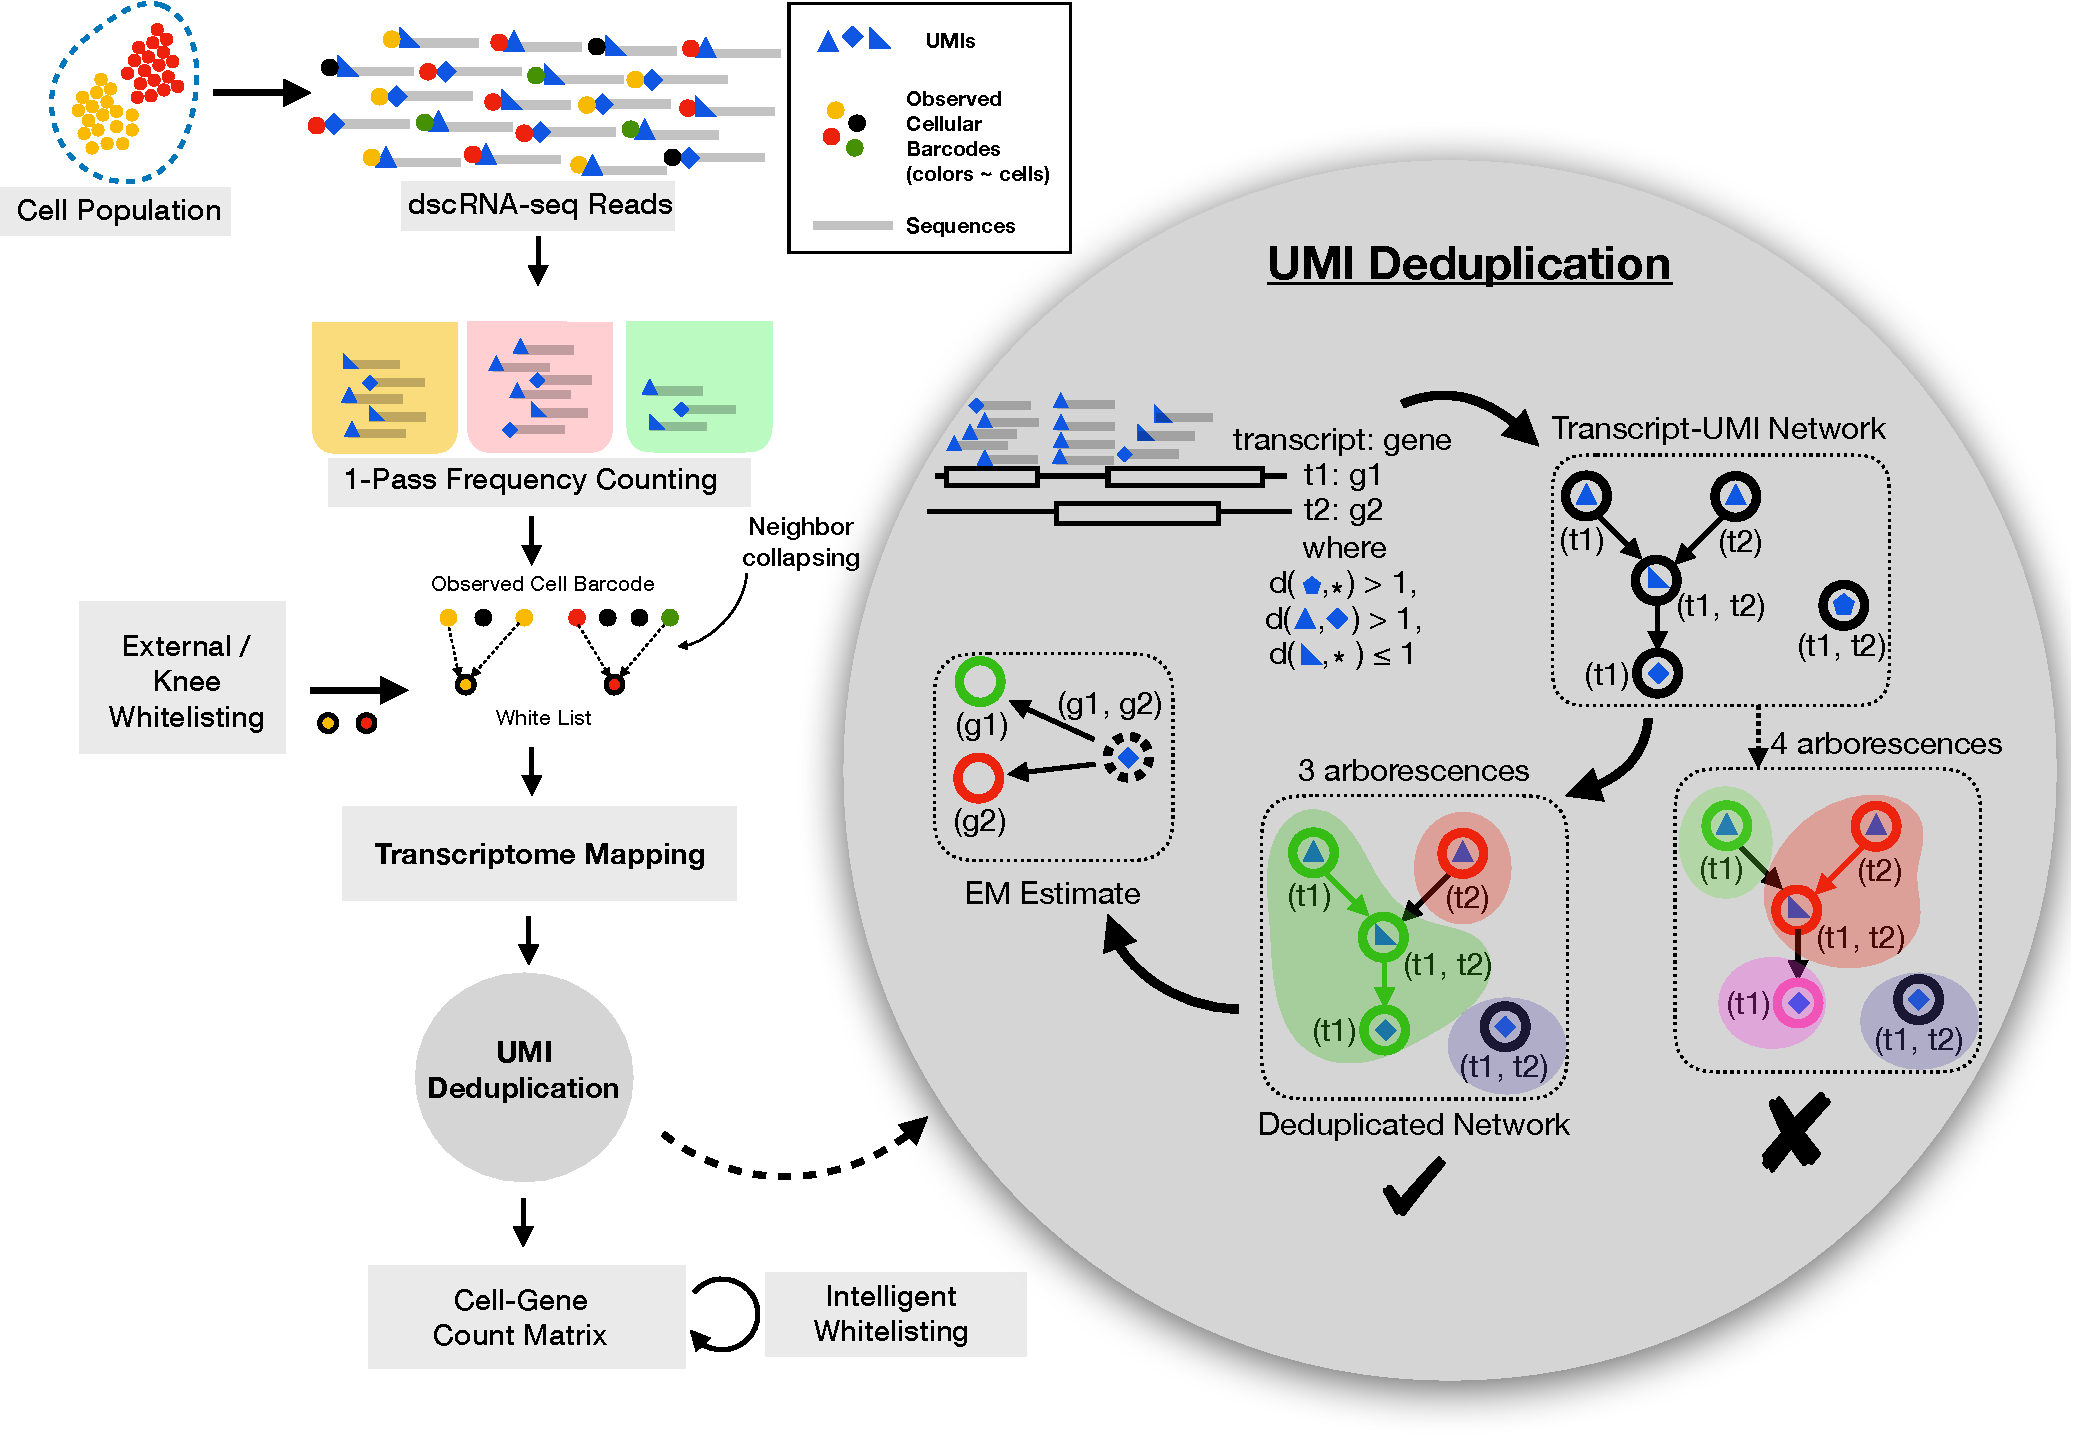
\includegraphics[width=1\textwidth]{alevin/alevin.pdf}
\caption{Overview of the \alevin pipeline. The input to the pipeline are sample-demultiplexed \texttt{FASTQ} files and there are several steps, outlined here, that are required to process this data and obtain per cell gene-level quantification estimates. The first step is cell-barcode (CB) whitelisting using their frequencies. Barcodes neighboring whitelisted barcodes are then associated with (collapsed into) their whitelisted counterparts. Reads from whitelisted CBs are mapped to the transcriptome and the UMI-transcript equivalence classes are generated. Each equivalence class contains a set of transcripts, the UMIs that are associated with the reads that map to each class and the read count for each UMI. This information is used to construct a parsimonious UMI graph (PUG) where each node represents a UMI-transcript equivalence class and nodes are connected based on the associated read counts. The UMI deduplication algorithm then attempts to find a minimal set of transcripts that cover the graph (where each consistently-labeled connected component --- each monochromatic arborescence --- is associated with a distinct pre-PCR molecule). In this way, each node is assigned a transcript label, and in turn, an associated gene label. Reads associated with arborescences that could be consistently labeled by multiple genes are divided amongst these possible loci probabilistically based on an expectation-maximization algorithm. Finally, optionally, and if not provided with high quality CB whitelist externally, an intelligent whitelisting procedure finalizes a list of high quality CBs using a na\"ive Bayes classifier to differentiate between high and low-quality cells.}
\label{fig:pipeline}
\end{figure}

The process of deduplication requires identifying duplicate reads based on their UMIs and alignment positions along the transcriptome. \Alevin uses a novel algorithm for deduplication that begins by constructing parsimonious UMI graphs, that we refer to as a PUGs, using information from the UMI sequences, the UMI counts and the transcript equivalence classes~\citep{mmseq}. This PUG is constructed such that each UMI-transcript equivalence class pair is represented by a node and there exists an edge from a node to any node that could have arisen from an amplified molecule due to sampling the underlying transcript (a single pre-PCR molecule) at a different position, or via a PCR or a sequencing error being introduced into the UMI.  When the direction of ``duplication'' during PCR is clear, a directed edge is added, otherwise a bi-directed edge is placed. An optimal covering of this graph, using the transcripts associated with each node, will give the minimum number of UMIs, along with their counts, required to explain the set of mapped reads. Hence, we have mapped the deduplication problem to that of finding a minimum cardinality covering of a given graph by monochromatic arborescences. Since the decision version of this problem is NP-complete, we propose a greedy algorithm to obtain a minimum cardinality covering of this graph (proof and algorithm detailed under Materials and Methods). Each covering, and the associated UMI, is assigned a set of transcript labels of size $\geq$ 1. After this UMI resolution phase, the remaining ambiguous reads with more than 1 transcript label, are assigned based on an expectation-maximization method~\citep{salmon}. 

Finally, having obtained per-cell gene expression estimates, CB whitelisting is finalized using a na\"ive Bayes classifier to differentiate between high and low-quality cells utilizing a set of features derived from the expression estimates and other diagnostic features~\citep{dropest}. In addition to the gene-by-cell count matrix, \alevin also provides information about the reliability of the abundance estimate computed for each gene in each cell in the form of a \emph{tier} matrix (and, optionally, the summarized variance of bootstrap estimates), which succinctly encodes the quality of the evidence used to derive the corresponding count.

\subsection{Impact of discarding multimapping reads}

\begin{figure}
  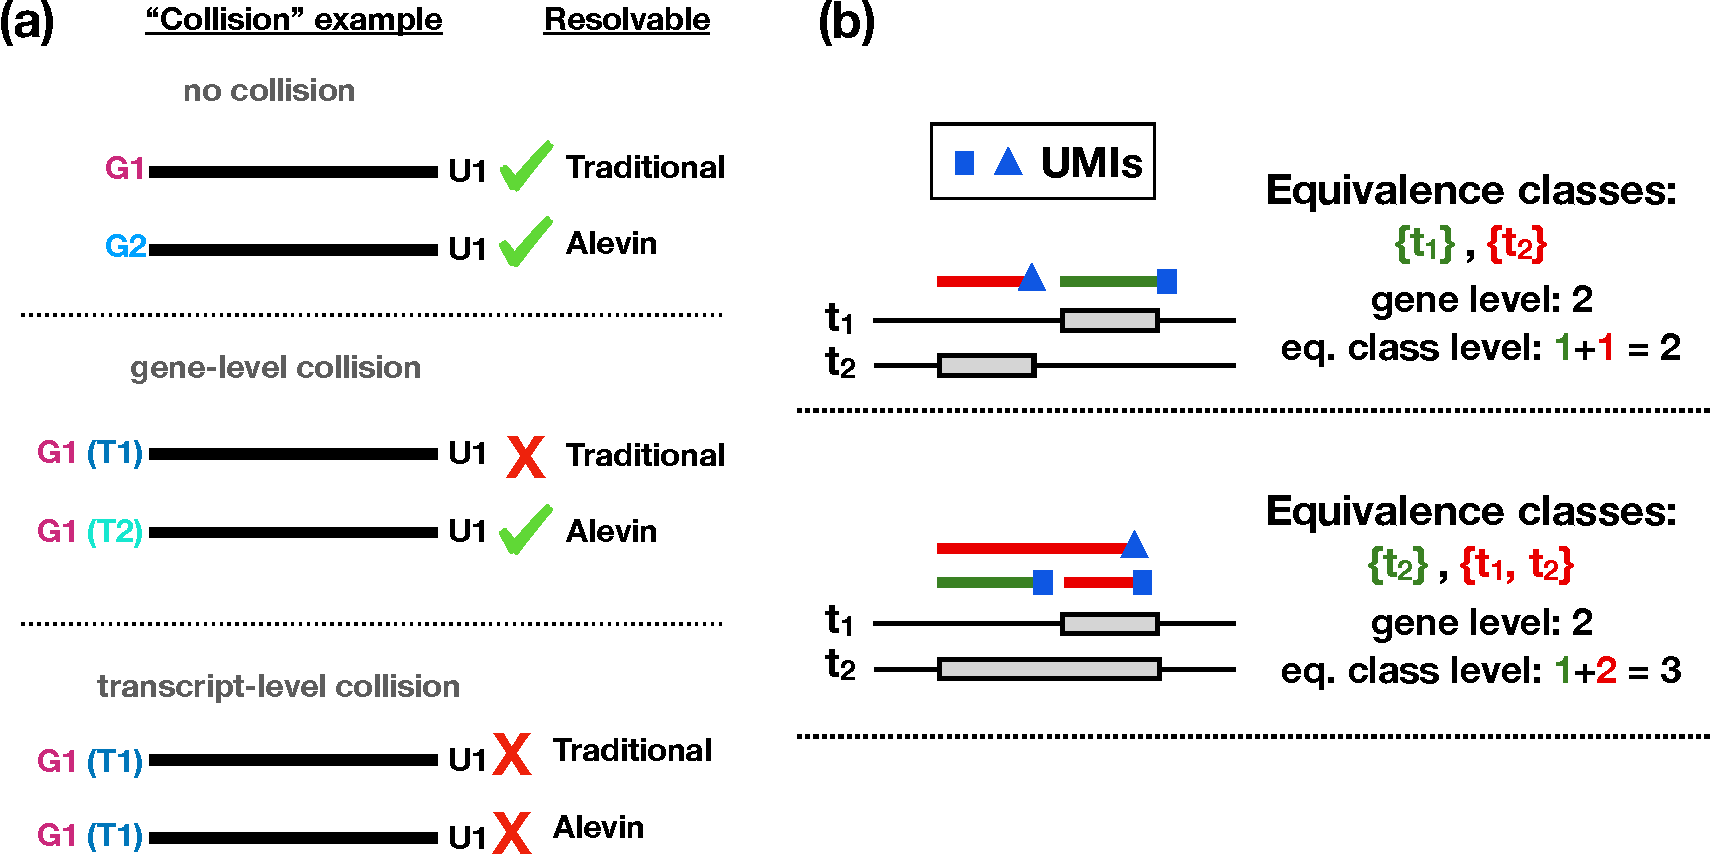
\includegraphics[width=\linewidth]{alevin/sims_combine_final.pdf}
  \caption{(a) This figure illustrates examples of various classes of UMI collisions, and which method(s) would be able to correctly resolve 
  the origin of the multimapping reads in each scenario. These cases are shown top-to-bottom in order of their likelihood. (b) A simulated example demonstrates how treating equivalence classes individually during UMI deduplication can lead 
  to under-collapsing of UMIs compared to gene-level methods (especially in protocols where the majority of cDNA amplification occurs 
  prior to fragmentation). In the first row, both methods report correctly a single UMI. In the second row, there are two fragmented molecules aligned against two transcripts from the same gene. The \alevin deduplication algorithm will attempt to choose the minimum number of transcripts required to explain the read mappings and hence correctly detect the UMI counts. The equivalence class method will over-estimate the gene count.}
  \label{fig:collision_sim}
\end{figure}

Before proceeding with a more detailed analysis of the \alevin pipeline, it is important to highlight scenarios where existing pipelines would fail using simple examples. These also lead to a better understanding of the \alevin UMI deduplication algorithm that intelligently utilizes transcript-level information to obtain accurate gene-level estimates. 
Since current deduplication methods do not have a mechanism to detect UMIs that map between multiple transcripts of the same gene, they can, in certain cases, incorrectly detect PCR duplicates and hence, under-estimate the total UMI counts. Some obvious cases can be resolved by considering the read-to-transcript mapping, instead of the read-to-gene mapping, as done in \alevin and shown in the left panel in \Cref{fig:collision_sim}.
The first row (top to bottom) demonstrates a case when we observe the same UMI (U1) being used to
tag transcripts from two separate genes (G1 and G2). Here, all methods are able to correctly assess that these instances of U1 are not 
PCR duplicates. In the center row, we observe the same UMI deriving from two (sequence-distinct) transcripts of the same gene. Here,
purely gene-level methods fail to resolve this collision, while \alevin's strategy can. Finally, in the bottom row, we observe a UMI 
collision within a single transcript. That is two different copies (molecules) of the same transcript have been tagged with the same UMI. 
This resolution cannot be resolved by any of the methods.  Though possible, the situation presented in the
third row is \emph{highly}-unlikely, especially given current sequencing depths.

A second scenario is highlighted in the right panel of \Cref{fig:collision_sim}
where using the transcript level equivalence classes lead to over-counting UMIs
(discussed further in Materials and Methods). In these simulated examples, different types of
transcripts, and corresponding expression patterns are shown. 
Reads are randomly sampled from the 3'-end of the
annotated-transcript(s) according to a realistic fragment length distribution,
where exon overlap induces the corresponding equivalence classes of each
fragment. The top simulation shows 1 (pre-PCR) molecule expressed for each transcript, 
identifiable by a unique-id (UMI), shown in blue. Due to the disjoint equivalence classes, both methods will
correctly assign the gene count. In the bottom simulation, both molecules originate from the second transcript. 
However, since the equivalence classes are different, the two fragments sharing a UMI will not be collapsed. 
Specifically, as the rate of splicing (and hence the number of equivalence classes) increases, so too does the number of distinct UMIs 
reported. In this case, the \alevin UMI deduplication algorithm will correctly detect the number of transcripts in order to greedily assign the minimum number of transcripts required to explain the given UMI and mapping information.

\begin{figure}
  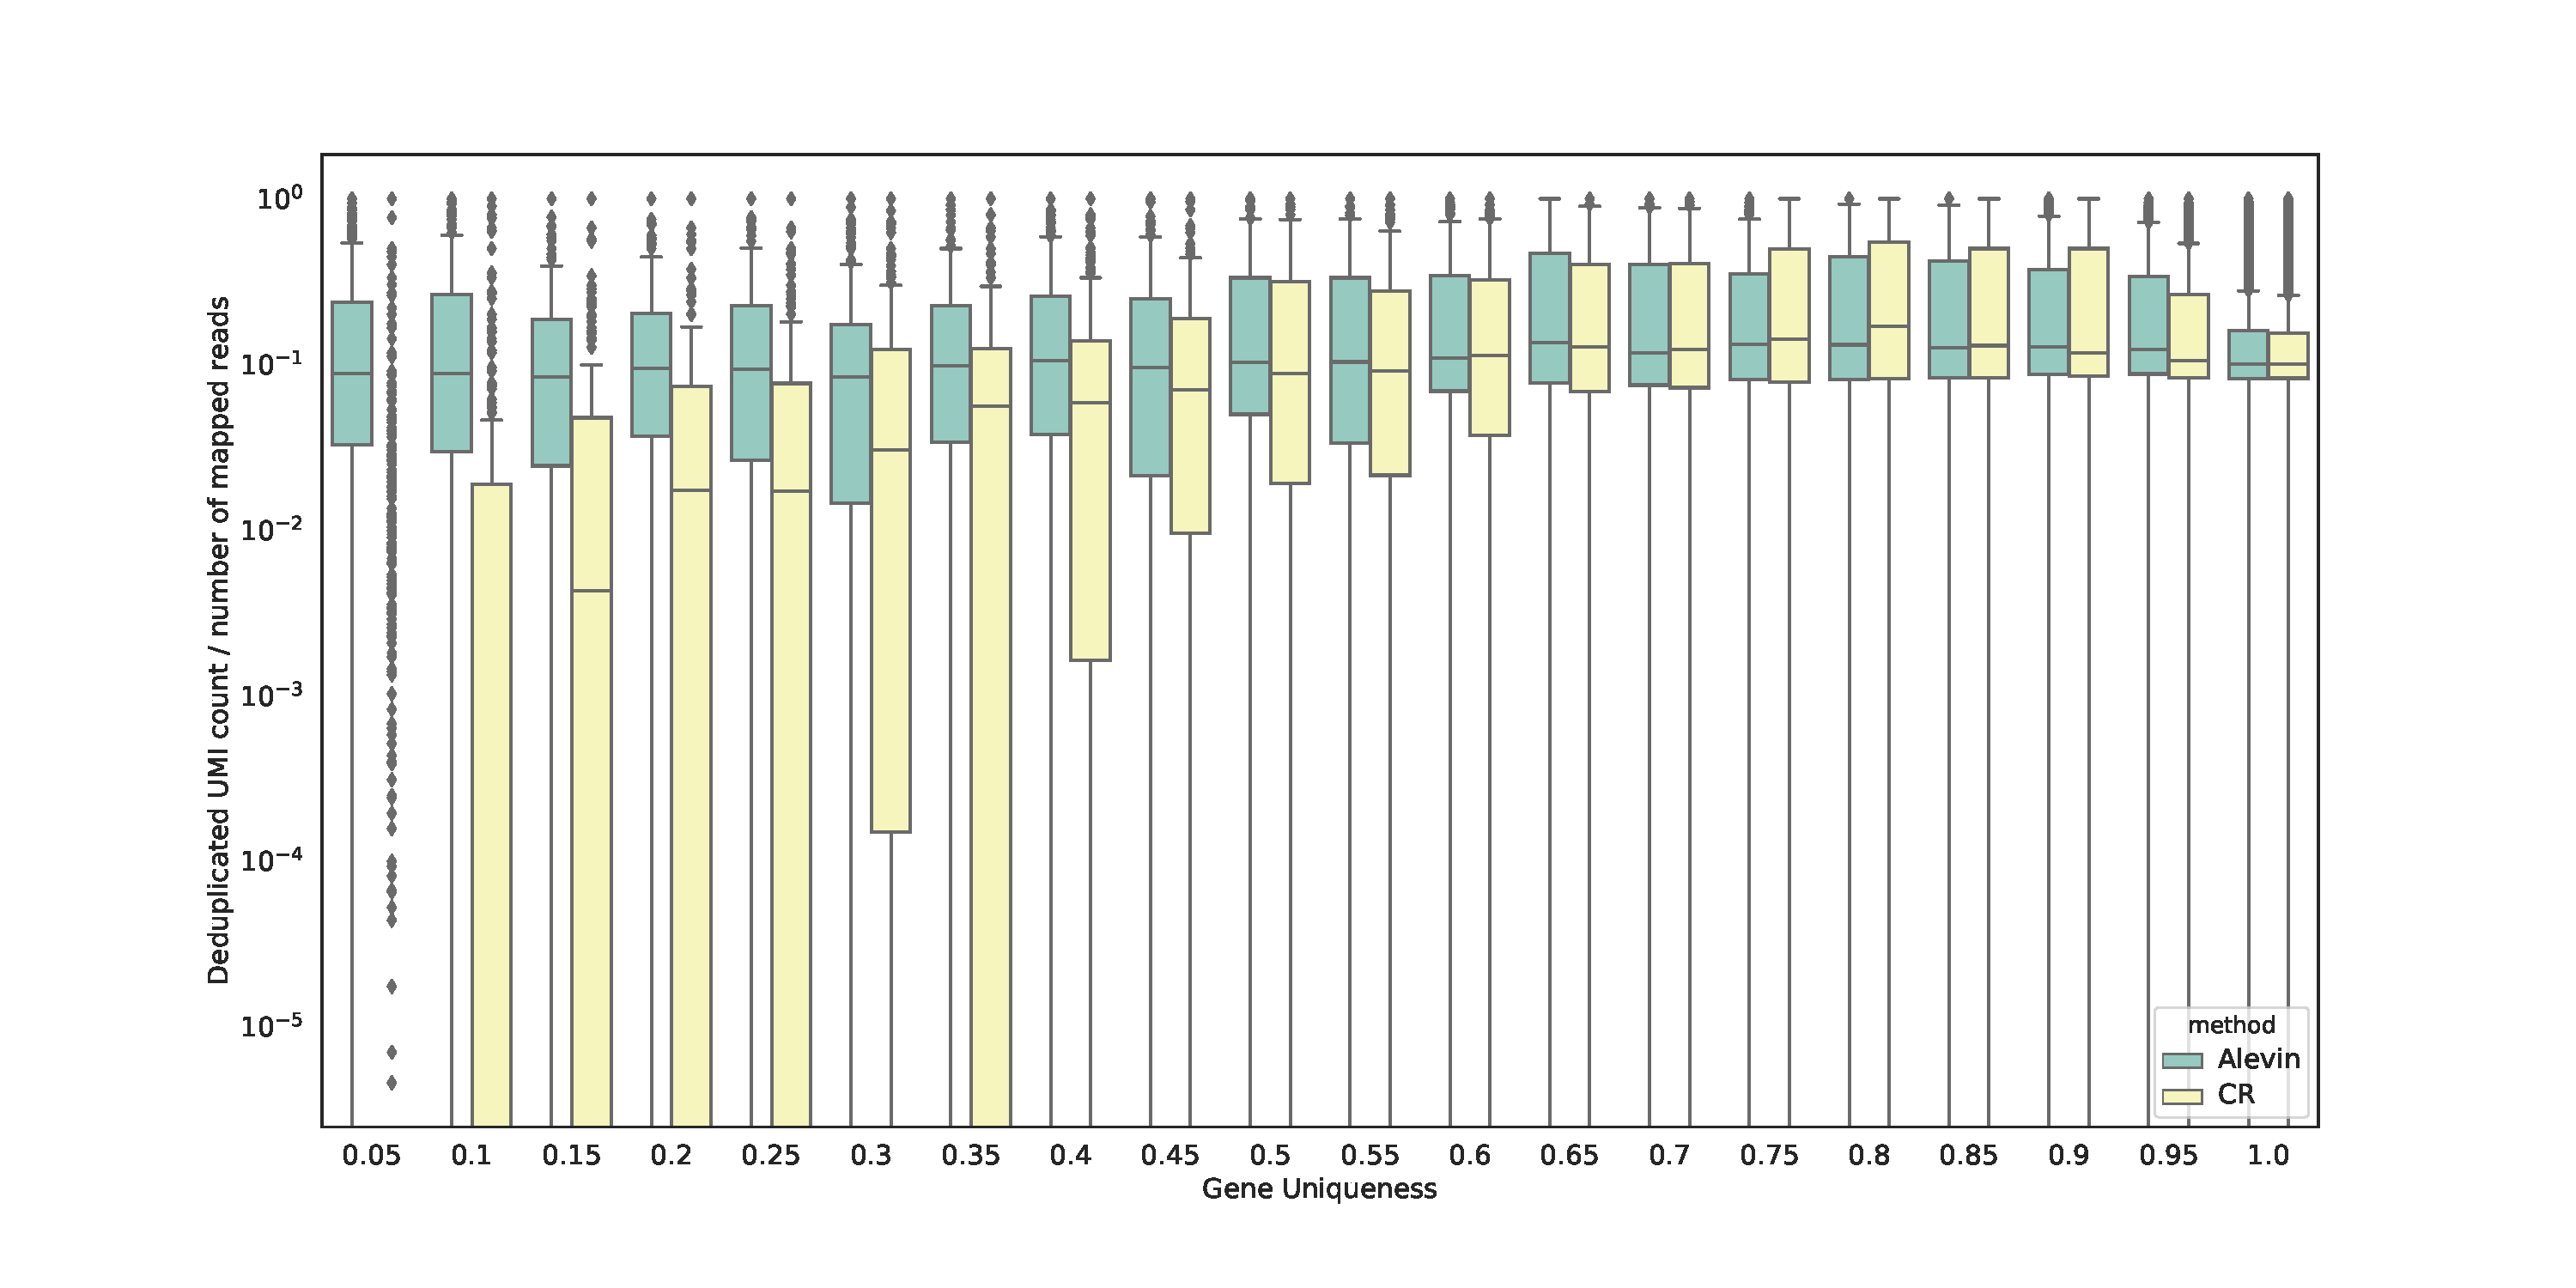
\includegraphics[width=\linewidth]{alevin/UMIdedup.pdf}
  \caption{The ratio of the final number of deduplicated
    UMIs against the number of initial reads for both \alevin and Cell Ranger (on the human PBMC 4k dataset)
    stratified by gene-level sequence uniqueness. The genes are divided into
    $20$ equal sized bins and the x-axis represents the maximum gene uniqueness
    in each bin. The plotted ratio for genes that have high sequence
    similarity with other genes is strongly biased when using \cellr. This is
    because \cellr will discard a majority (or all) of the reads originating
    from these genes since they will most likely map to multiple positions
    across various genes. \Alevin, on the other hand, will attempt to accurately
    assign these reads to their gene of origin. This plot also demonstrates that \alevin does not over-count UMIs,
    which would be the case if deduplication was done at the level of equivalence classes.}
  \label{fig:umidedup}
\end{figure}

To show that the UMI deduplication algorithm from \alevin does, indeed, perform better, we calculate the ratio of the number of reads mapping to each gene and the final count of UMIs as predicted by \alevin and \cellr for that gene. When a read maps ambiguously, the count is divided uniformly between the genes. Hence, if a read maps to two genes, the count for each is incremented by $0.5$ to get the initial number of reads mapping to these genes. Note that the mappings are also different under each pipeline and that some reads may be inherently ambiguous under one or both mappings. These reads cannot be accurately assigned but, while \cellr discards them, \alevin assigns them to a gene via the PUG-resolution algorithm, or,in the case that parsimony fails to distinguish a single best gene, proportionally to multiple genes according to the other uniquely-mapping reads of the experiment.  We divide the genes into 20 bins, based on the number of k-mers shared across genes. We expect the above calculated ratio to remain fairly consistent across these 20 bins, irrespective of the sequence properties of the genes in them. However, we observe in \Cref{fig:umidedup}, that the predictions from \cellr are biased for the genes with low sequence uniqueness. This is because a large number of reads from these genes will multimap across genes and will, therefore, be discarded. Hence, simply discarding multimapping reads seems to bias the count estimates for all genes but strongly impacts counts for genes that are expected to have a larger number of multimapping reads due to their high sequence similarity. 

\subsection{Accuracy analysis on real datasets}
\begin{table}[htb]
\centering
\caption{Number of final whitelisted cellular barcodes output by \alevin and \cellr.}
      \begin{tabular}{cccc}
        \hline
           Dataset & \cellr  & \Alevin & No.of reads \\ \hline
    Human PBMC 4k & 4346 & 4341 & 379,462,522\\
    Human PBMC 8k & 8379 & 8291 & 784,064,148\\
    Mouse Neurons 900 & 933 & 1291 & 52,805,264 \\
    Mouse Neurons 2k & 2009 & 1881 & 147,010,995 \\
    Mouse Neurons 9k & 9116 & 8519 & 383,366,284 \\ \hline
      \end{tabular}
      \label{suptab:whitelist}
\end{table}

To assess the performance of \alevin, both in terms of accuracy in quantification and resource consumption, we ran it on 10x Chromium datasets from human and mouse. We compare our results against the \cellr pipeline\citep{tenx}, the \dropest pipeline\citep{dropest} \footnote{Note that we were not able to run the dropEstr Bayesian correction method and the results presented are after running just the \dropest pipeline~\citep{dropseqsrc}.}. , and a custom pipeline, with an external list of whitelisted CBs, using STAR\citep{star}, featureCounts \citep{featurecounts}, and UMI-tools \citep{umitools}, which we refer to as the \naive pipeline. The exact parameters for running each tool are provided under Materials and Methods. Note that we run \alevin with the \texttt{{--}keepDuplicates} flag during indexing, which ensures that even when multiple sequence-identical transcripts exist in the annotation, they are not discarded. This is to allow for fair comparison against the other tools, since they do not discard such transcripts, and the existence of such transcripts will impact the number of multimapping reads. However, we do not generally recommended using this flag when running \alevin. We observe that the number of final whitelisted cells predicted by \alevin are in close proximity to the count of cells predicted by \cellr (and \dropest, since they use the same whitelise), but there are non-trivial differences (\Cref{suptab:whitelist}). Comparison on data using the Drop-seq\citep{dropseq} protocol is also detailed below. Comparisons against the recently released version 3.0.0 of \cellr are also provided (Additional file 1: Figure S1), along with results from another run of \alevin using different parameters. Where mentioned, the results are stratified by gene uniqueness which is the proportion of k-mers, of size 31, that are not shared between two or more genes. We note that varying the k-mer size changes the stratification of the genes but does not impact the overall correlation and performance of the methods. We show this for the mouse neuronal 900 dataset (Additional file 1: Figure S2). We calculated this for each gene in the human (GENCODE release 27, GRCh38.p10) and mouse (GENCODE release M16, GRCm38.p5) transcriptomes. Note that this was not calculated using the canonicalized k-mers from the genes. This is because the \scrnaseq protocols are stranded and a read, therefore, can not multi-map between two genes if the reverse complement of one of them is shared with the other's forward sequence. 

\subsection{Accuracy of estimates against bulk data}
\begin{table}[htb]
\centering
\caption{Average Spearman correlation of gene-level estimates from each method for the single cell datasets against bulk data from the same cell types (4 for human, 3 for mouse).}
      \begin{tabular}{ccccc}
        \hline
           Dataset & \Alevin & \cellr & \naive & \dropest \\ \hline
           Human PBMC 4k & 0.813 & 0.780 & 0.747 & 0.783 \\
           Human PBMC 8k & 0.810 & 0.772 & 0.740 & 0.776 \\
           Mouse Neurons 900 & 0.812 & 0.773 & 0.761 & 0.779 \\
           Mouse Neurons 2k & 0.822 & 0.781 & 0.767 & 0.784\\
           Mouse Neurons 9k & 0.831 & 0.796 & 0.776 & 0.803 \\ \hline
      \end{tabular}
      \label{suptab:fullcorr}
\end{table}

To test the accuracy of the quantification estimates, we aggregate the estimates from each of the single-cell quantification tools (summing across all cells) and calculate the correlation with estimates predicted by RSEM\citep{li2011rsem} (paired with Bowite2\citep{bowtie2} alignments) using bulk datasets from the same cell types. While the differences between single-cell and bulk sequencing protocols and techniques are significant, we believe that, in the absence of established benchmarks, the correlation between them is a reasonable indicator of the accuracy of each quantification method. Estimates from \alevin, when summed across all cells, have a higher Spearman rank correlation than the \cellr, \dropest, and \naive pipelines (\Cref{suptab:fullcorr}).  Specifically, we posit that the methods demonstrate a strong and persistent bias against groups of two or more genes that exhibit high sequence similarity.  That is, the more sequence-similar a gene is to another gene, the less likely these pipelines are able to assign reads to it --- in the extreme case, some genes essentially become \emph{invisible} due to the \emph{in silico} biases of these approaches (a similar effect was reported by Robert and Watson ~\citep{makemickhappy} in bulk RNA-seq data when simple read-counting approaches are used for quantification, where they highlight that many such genes are relevant to human disease).

\begin{figure}
\centering
    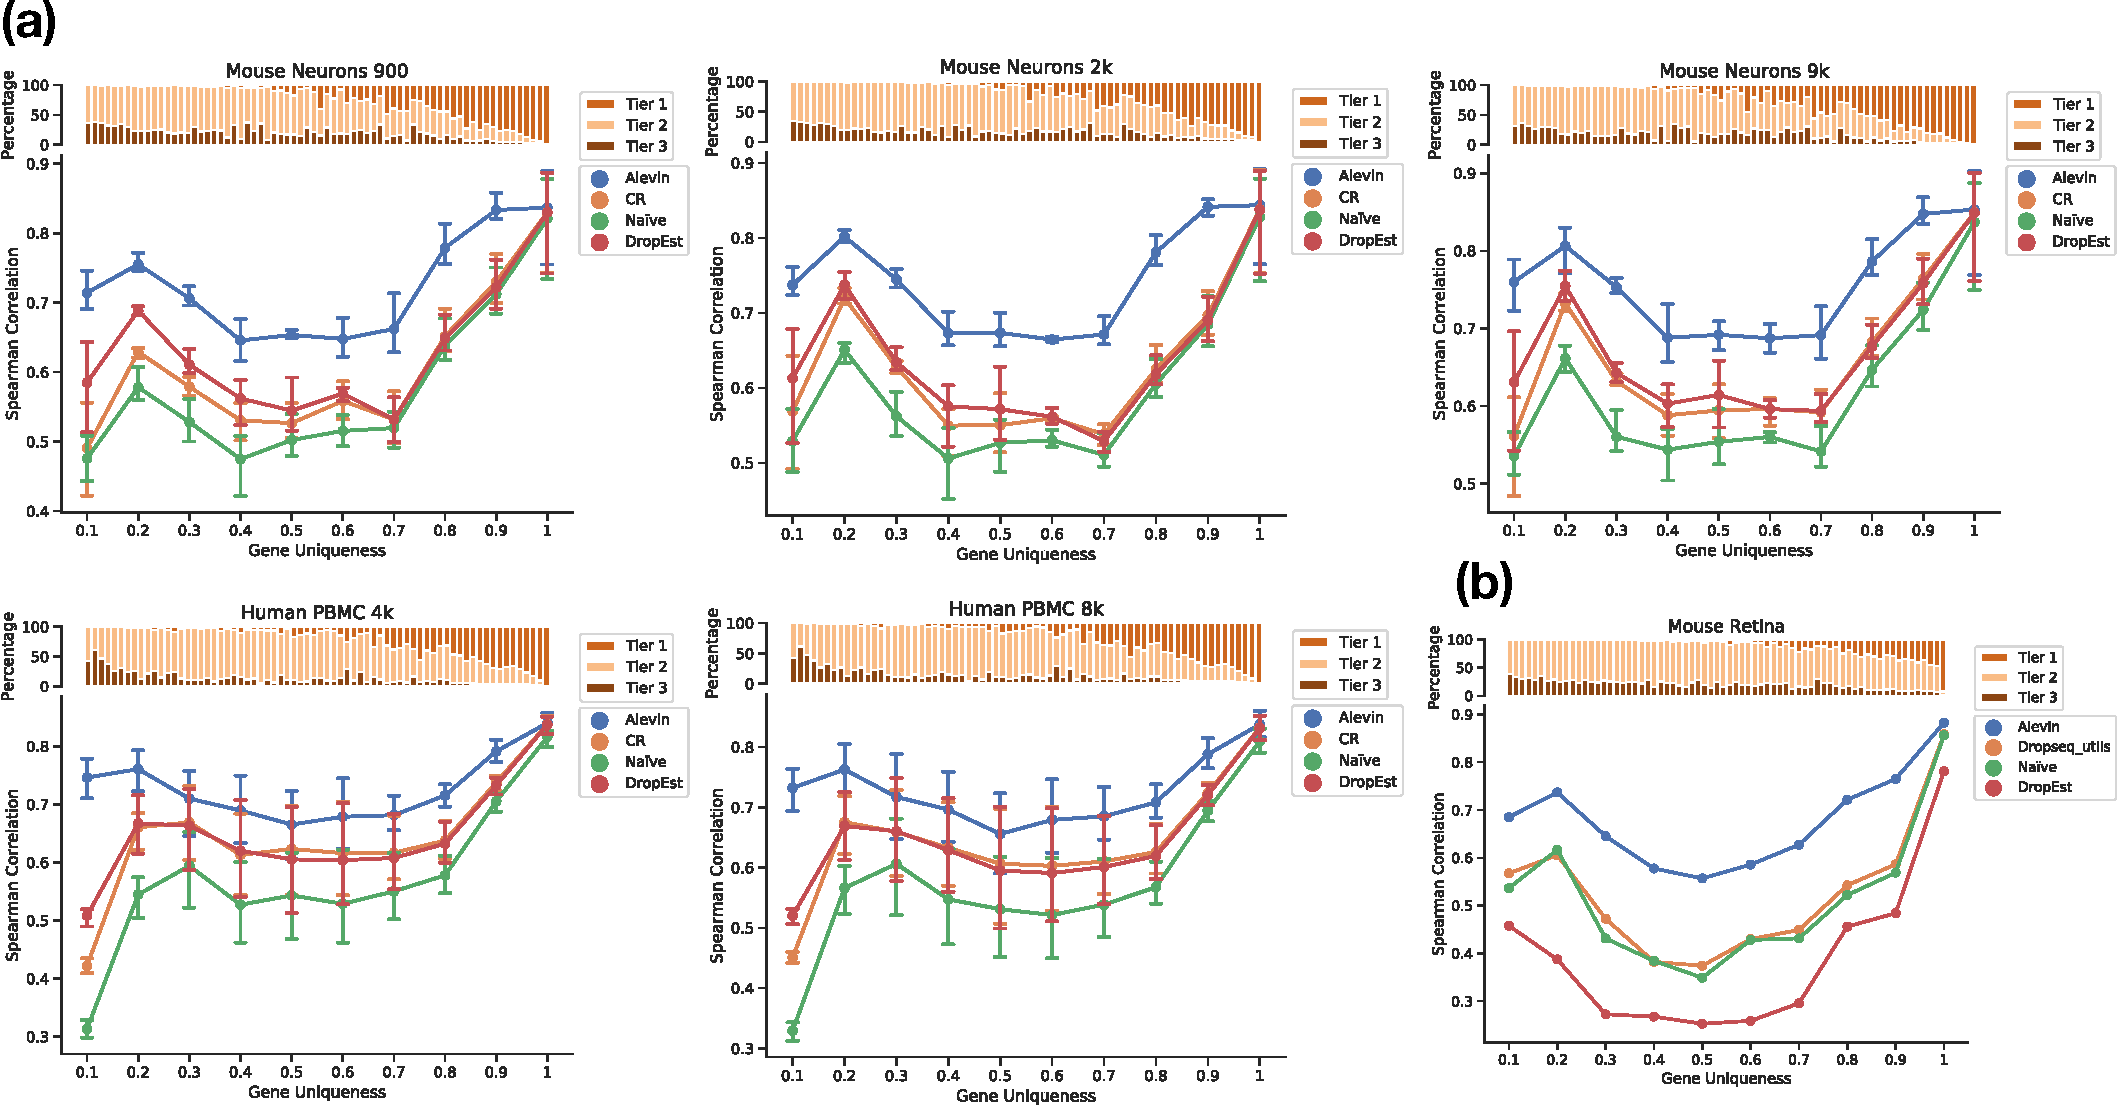
\includegraphics[width=\linewidth]{alevin/combine_corr.pdf}
  \caption{(a) The Spearman correlation between quantification estimates (summed across all cells) from different \scrnaseq methods against bulk data from the mouse neuronal and human PBMC datasets, stratified by gene sequence uniqueness. The bar plot on the top of each figure shows the percentage of genes in each bin that have unique read evidence. Tier 1 is the set of genes with only uniquely mapping reads. Tier 2 is genes that have ambiguously mapping reads, but are connected to unique read evidence that can be used to resolve the multimapping reads. Tier 3 is  genes that are completely ambiguous. Note that all methods perform very similarly on genes from tier 1, but the performance of \alevin is much better for the other tiers. (b) Comparison of various methods used to process dropseq data from mouse retina with 4k cells. The Spearman correlation is calculated against bulk quantification estimates predicted using Bowtie2 and RSEM on data from the same cell type.}
  \label{fig:correlation}
\end{figure}

\begin{table}[htb]
\centering
\caption{Number of genes in each bin, when stratified by gene uniqueness.}
      \begin{tabular}{ccc}
        \hline
           Bin number & Human  & Mouse \\ \hline
    1 & 3155 & 4786 \\
    2 & 894 & 1089 \\
    3 & 853 & 945 \\
    4 & 822 & 1061 \\
    5 & 962 & 1104 \\
    6 & 1174 & 1318 \\
    7 & 1565 & 1476 \\     
    8 & 2546 & 1877 \\ 
    9 & 4695 & 2960 \\ 
    10 & 41622 & 36763 \\ \hline
      \end{tabular}
      \label{suptab:bin_sizes}
\end{table}

To further explore this hypothesis, we stratified the accuracy of the different methods by the uniqueness of the underlying genes (\Cref{fig:correlation}a, \Cref{suptab:bin_sizes}). The bar plots at the top of each subfigure represent the tiers of the genes as assigned by \alevin. Tier 1 is the set of genes where all the reads are uniquely mapping. Tier 2 is genes that have ambiguously mapping reads, but connected to unique read evidence as well, that can be used by the EM to resolve the multimapping reads. Tier 3 is the genes that have no unique evidence and the read counts are, therefore, distributed between these genes according to an uninformative prior. In agreement with the hypothesized relationship, we observed that the higher accuracy of \alevin is particularly large for genes with a lower proportion of unique k-mers, that tend to belong to tier 2 or 3. On genes from tier 1, all the methods to perform similarly. Thus, the approach of \cellr, \dropest, and \naive, which discard reads mapping to multiple genes, results in systematic inaccuracies in genes which are insufficiently unique (i.e. which share a high degree of sequence homology with some other gene). 

\begin{figure}
  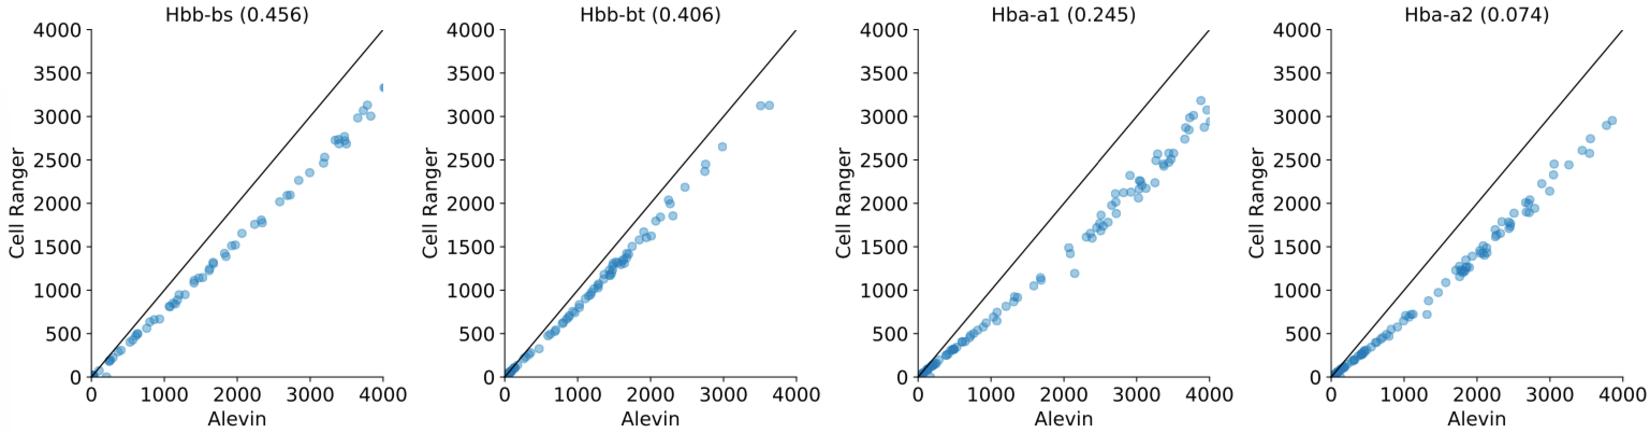
\includegraphics[width=\linewidth]{alevin/hbgene.pdf}
  \caption{Expression of the Hba and Hbb genes as predicted by \alevin and \cellr in mouse neuronal cells. The title of each plot is the name of the gene and its k-mer uniqueness ratio. Note that \cellr systematically underestimates the expression of these genes compared to \alevin. This bias is greater for the Hba genes, which have a lower uniqueness ratio, and therefore, a greater number of multi-mapping reads.}
  \label{fig:hbgene}
\end{figure}

\begin{figure}
    \centering
  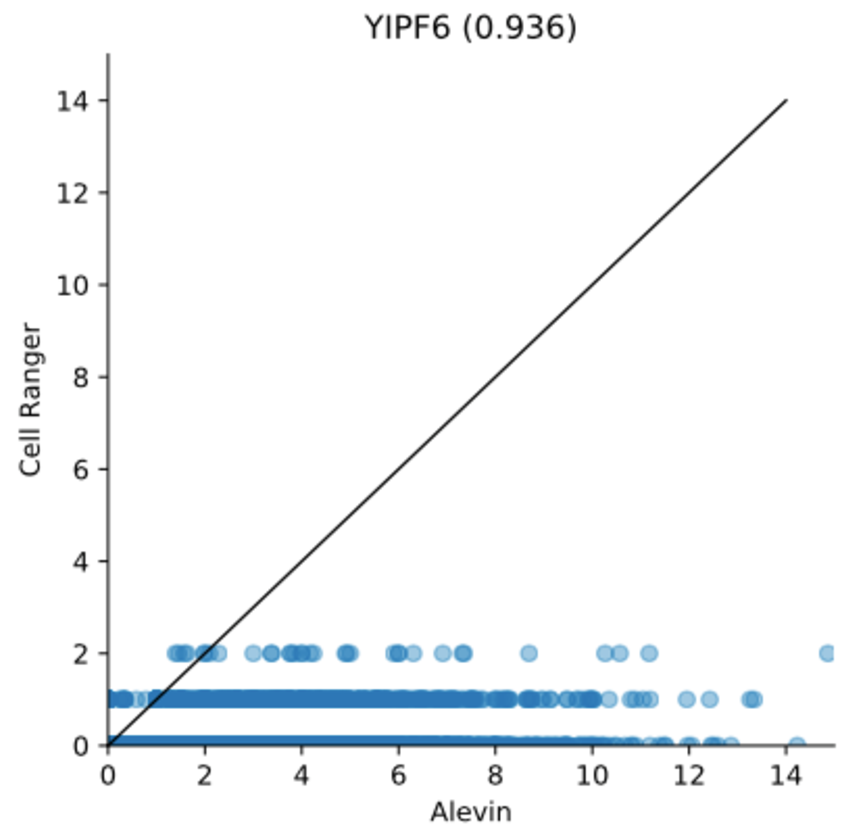
\includegraphics[width=0.3\linewidth]{alevin/yipf6gene.pdf}
  \caption{Expression of the YIPF6 gene (which has a high uniqueness ratio) as predicted by \alevin and \cellr in the PBMC8k data.}
  \label{fig:yipgene}
\end{figure}

This bias could impact the expression estimates of important marker genes, such as the genes for the hemoglobin alpha and beta proteins in the mouse neurons\citep{han2018mapping, richter2009neurons}. Due to their lower uniqueness ratio, \cellr appears to exhibit a bias against such genes, and their expression, as predicted by \alevin, is systematically higher (\Cref{fig:hbgene}).  Anecdotally, we also noticed that, in the human PBMC data, \alevin sometimes predicts the expression of even relatively sequence-unique genes, like YIPF6, that we expect to be expressed in a subpopulation of these cells (monocytes)~\citep{yipf6}, but which exhibit almost no expression as predicted by \cellr (\Cref{fig:yipgene}).  Because the bias against sequence-ambiguous genes is fundamental and sequence-specific, it cannot be easily remedied with more data, but instead requires the development of fundamentally novel algorithms, like \alevin, that account for, rather than discard, reads mapping to such genes. Hence, \alevin not only quantifies a greater proportion of the sequenced data than existing methods, but also does so more accurately and in a less-biased manner.

\subsection{Accuracy of estimates using combined genomes}
To further assess the accuracy of quantification estimates, in the absence of
  any established read-level simulation protocol, we performed an experiment aimed
  to introduce controlled gene-level multimapping to analyze its effect on the
  different methods.  We quantified the mouse neuronal 900 sequencing dataset
  using both \cellr and \alevin and each quantification was performed under
  two separate references: the mouse genome, and the combined human and mouse genome.
  Noting that the reads in this experiment originate from mouse, we
  desire that the quantifications returned by a method deviate as little as
  possible under the two different reference configurations. Under ideal
  conditions, for example, the gene counts under both references should be the
  same. However, combining the mouse and human references increases the gene
  sequence ambiguity, due to the presence of homologous genes, resulting in
  misestimation. 
  
  \begin{figure}
      \centering
    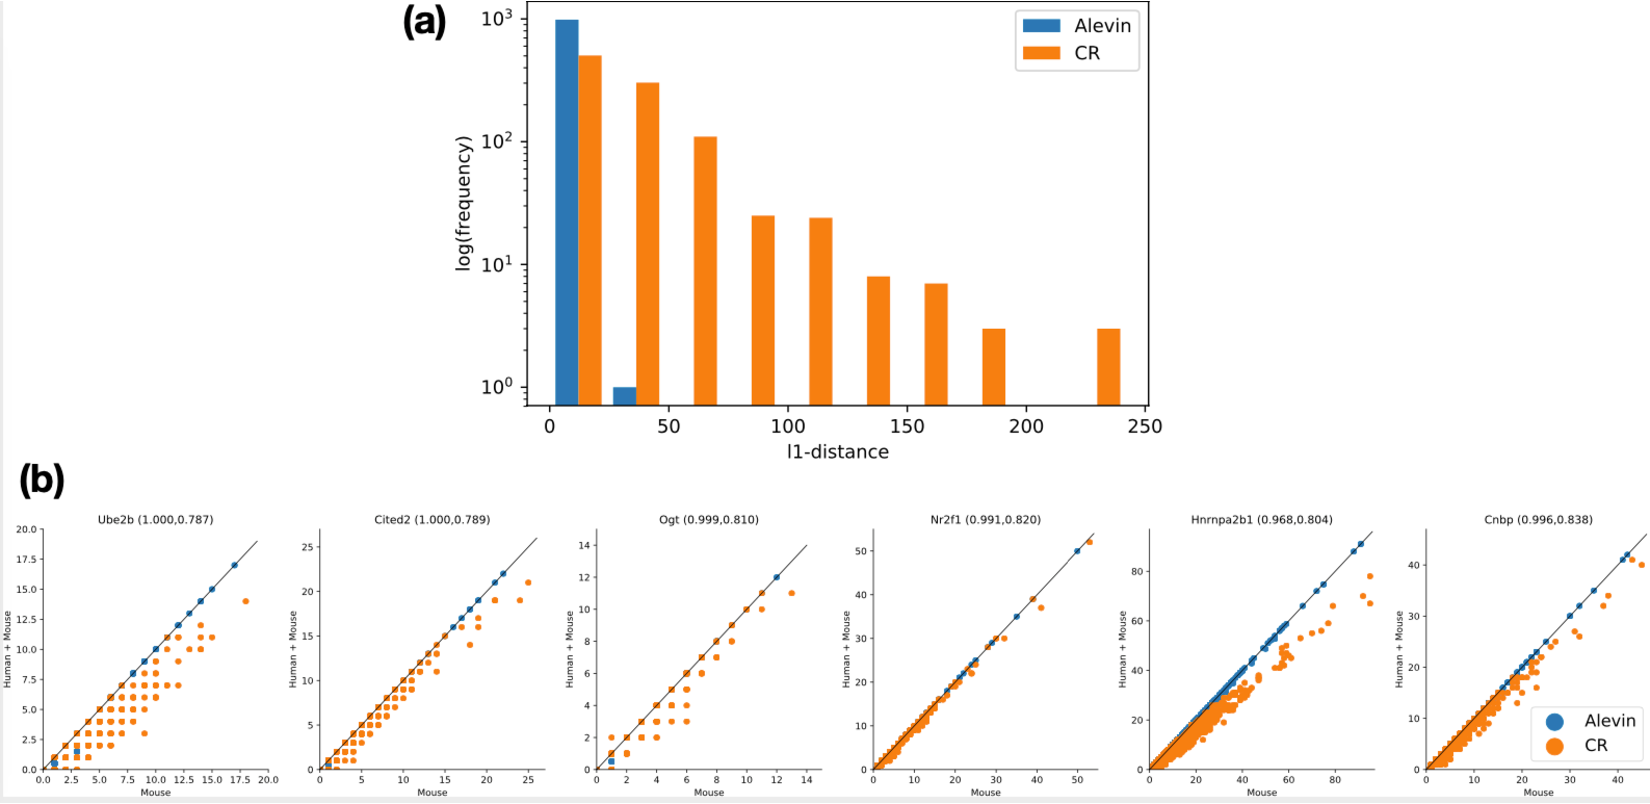
\includegraphics[width=\linewidth]{alevin/mixed_combine.pdf}
    \caption{(a) Histogram of the $\ell_{1}$ distance between the
        quantification estimates of tools on the mouse neuron 900 data, when run
        using different references for quantification (just mouse versus mouse and
        human). Results are presented for both \alevin and \cellr. Since, in
        reality, all reads are expected to originate from mouse, deviations from
        quantifications under the only mouse reference signify misestimation ---
        often due to the introduction of sequence-similar genes in the human
        genome. \Alevin is able to resolve this ambiguity well, while \cellr
        instead discards such reads, leading to different quantification estimates
        under the two references. (b) Counts for the topmost genes that have high sequence homology between human 
        and mouse but are sequence unique in the mouse reference. The title of each plot is the gene name 
        along with the sequence uniqueness ratio under just the mouse reference and under the joint reference. Hence, the
        \cellr counts decrease across cells when the gene uniqueness decreases. Note that these genes were filtered such
        that they have $>$100 count difference for either \alevin or \cellr when summed across all cells. }
    \label{fig:mixedanalysis}
  \end{figure}
  
  We show in \Cref{fig:mixedanalysis}a that the distance under
  the two references is higher for the \cellr estimates than that for the
  \alevin estimates. Due to the increased homology among genes between the
  references, the ratio of reads mapping to multiple genes increases, resulting
  in more information being discarded by \cellr. The total number of UMIs
  accounted for by \cellr decreases by $\sim20,000$, in comparison the number of
  distinct UMIs predicted by \alevin decreased by $\sim1,500$, which one might
  attribute to changes in the underlying PUGs as a result of mapping
  $\sim0.01\%$ more reads. The number of human genes expressed (non-zero UMI count)
  under the joint reference is $624$ for \cellr and $600$ for \alevin, out of a total of $58,288$ genes. 
  Note that in both cases, these genes account for $<0.05\%$ of the total UMI count predicted by each 
  method.

  To provide a statistical analysis of the differences observed for the methods
  under the two different reference sequences, we performed the following test.
  We sample, randomly, $1000$ sets of $100$ cells from the entire experiment,
  and for each sample, we compute the sum of absolute difference between the
  predictions of each tool under both references. We compare the resulting
  distribution of differences for \cellr with that of \alevin and find that the
  differences in \alevin's quantifications are smaller than those of \cellr ($p < 0.001$, Mann Whitney Wilcoxon test). 
  These distributions are plotted in Additional file 1: Figure S3.

 We also show in \Cref{fig:mixedanalysis}b that, for the genes that have
  sequence similarity in the joint reference but are unique in the mouse genome,
  \cellr expression estimates vary much more than those from \alevin.

\subsection{Time and memory efficiency}
The time and memory requirements for \alevin are significantly less than those for the existing pipelines (\Cref{fig:timemem}), where all methods were run using $16$ threads. \dropest is excluded from the figure since it consumes the BAM file output by \cellr and is not a complete end-to-end pipeline. For the smallest dataset (900 mouse neuronal cells), \alevin was $\sim5$ times faster than \naive and $\sim21$ times faster than \cellr. This difference increases further as the size of the dataset increases, since the performance of \alevin scales better than the other tools. Hence, where \alevin took only $70$ minutes to process the human PBMC 8k dataset, \cellr took $22$ hours and \naive took $11$ hours. On this dataset, \dropest took $\sim2$ hours, after \cellr was used to process and align the reads. In terms of memory, \alevin used only $\sim13$GB on the human PBMC 8k cell dataset, whereas \naive took $\sim20$GB and \dropest took $\sim32$GB. For the mouse neuronal 9k cell dataset, \alevin used $\sim14$GB, \naive  $\sim18$GB, and \dropest $\sim52$GB. In both cases, \cellr required a minimum of 16GB just for STAR indexing. We note that \cellr allows the user to specify a maximum resident memory limit, and we ran \cellr allowing it to allocate up to 120GB so that the extra runtime was not due to limitations in available memory. We also note that for \dropest, we were not able to run the Bayesian collision correction algorithm implemented in dropEstr; however, given the relatively long UMI tags employed in chromium V2 chemistry compared to inDrop, one would expect the effect of this extra phase to be limited anyway.

\begin{figure}
    \centering
  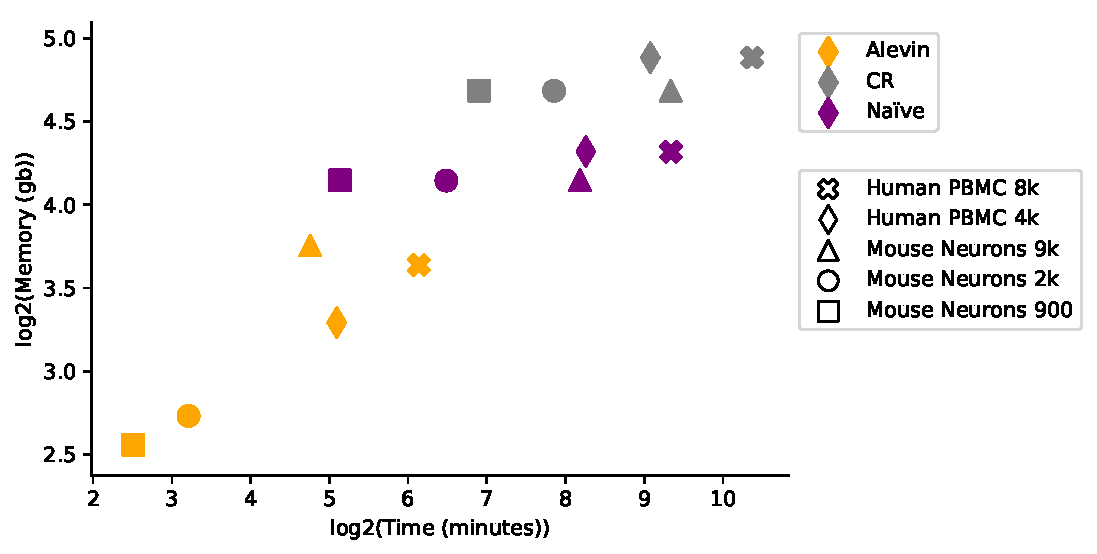
\includegraphics[width=\linewidth]{alevin/timing.pdf}
  \caption{The time and memory performance of the different pipelines on the five datasets. \Alevin requires significantly less time and memory than the other pipelines. Note that for \cellr, the memory plotted is the lower bound, which is the size of the index and the actual memory usage can be much higher.} %(b) The time and memory usage of \alevin using different number of threads. The runs for each dataset were repeated using $5, 10, 15,$ and, $20$ threads.}
  \label{fig:timemem}
\end{figure}

We observe that the optimal number of threads for running \alevin is $10-12$, where the maximum gain in terms of time and memory is achieved. \Alevin is designed to make efficient use of multiple threads, though the optimal number of threads can depend on many factors, such as the speed of the underlying disk and the size of the raw input and output matrix to be written. While runtime decreases with the number of threads uses, the memory profile changes very little as threads are added. 

\subsection{Comparison on DropSeq data}
In addition to data generated using the 10x chromium protocol\citep{tenx}, we 
also tested \alevin on mouse retina data generated using the Drop-seq protocol~\citep{dropseq}. 
We compare \alevin against UMI-tools (the \naive pipeline    
from the main paper), \dropest, and dropseq\_utils~\citep{dropseq} --- the processing    
pipeline originally used by~\citet{dropseq}.   
 Again, we compared the correlation of gene abundances, summed across all cells    
and as produced by the different methods with the estimates from bulk    
data~\citep{mouse_retina} in the same tissue (\Cref{fig:correlation}b). We observe a    
similar trend across gene-uniqueness bins as was observed for the 10x datasets.    
\Alevin demonstrates higher correlation, overall, with the bulk data, and the    
improvements are particularly substantial for genes that are not    
sequence-unique. Further, \alevin is much faster, and takes less memory than    
the other pipelines. \Alevin took $17$ minutes to process this data, which is much faster than the UMI-tools-based    
pipeline ($\sim3.2$ hours), the dropseq\_utils-based pipeline ($\sim15.5$    
hours), and even \dropest ($25$ minutes). The memory usage of \alevin was $6.5$GB, which is less than half the    
memory usage of the closest tool (UMI-tools at $17.72$GB).
The dropseq\_utils-based pipeline took $25.07$GB and while \dropest used
$10.8$GB, that does not include the memory consumed by \cellr to index the reference and align reads against it to
produce the BAM file.
While \alevin has been primarily designed and tested with 10x data in mind, the method
is generic for droplet-based tagged-end protocols, and we observe that it also seems to perform
well on Drop-seq data. 

\section{Conclusion}
We present a new end-to-end pipeline for performing gene-level quantification
from \dscrnaseq that is accurate, efficient, and easy to use. Our method,
\Alevin, relies on a new formulation of the UMI-resolution problem that both
accounts for transcript-level constraints on how UMIs may have been generated
and that allows resolving the potential origin of a UMI even when the
corresponding reads map between multiple genes.

Our analyses demonstrate that, compared to \cellr (and \naive), \alevin achieves
a higher accuracy, in part because of considering a substantially larger number
of reads. Further, \alevin is considerably faster and uses less memory than
these other approaches. These speed improvements are due to a combination of the
fact that \alevin uses bespoke algorithms for CB and UMI edit distance
computation, read mapping, and other tasks, and is a unified tool for performing
all of the initial processing steps, obviating the need to read and write large
intermediate files on disk. These optimizations make it possible to efficiently
process \dscrnaseq datasets on commodity computers reducing computational
barriers to processing and re-processing of such data.

In the future, we hope to further improve the benchmarking of accuracy
  for single-cell quantification and barcode whitelisting approaches, as the
  lack of standard benchmarks makes the assessment of new methods difficult. We
  also hope to explore alternative cell barcode whitelisting and PUG resolution strategies --- for example,
  adopting a generative model for PCR and sequencing error and seeking a maximum
  likelihood rather than maximum parsimony-based resolution of the PUGs.

